%% Template originaly created by Karol Kozioł (mail@karol-koziol.net) and modified for ShareLaTeX use

\documentclass[a4paper,11pt]{article}

\usepackage[T1]{fontenc}
\usepackage[utf8]{inputenc}
\usepackage{graphicx}
\usepackage{xcolor}


\usepackage{tgheros}
\usepackage[defaultmono]{droidmono}

\usepackage{amsmath,amssymb,amsthm,textcomp}
\usepackage{enumerate}
\usepackage{multicol}
\usepackage{tikz}
\usepackage{subcaption}
\usepackage{geometry}
\geometry{left=25mm,right=25mm,%
bindingoffset=0mm, top=20mm,bottom=20mm}




\newcommand{\linia}{\rule{\linewidth}{0.5pt}}

% custom theorems if needed
\newtheoremstyle{mytheor}
    {1ex}{1ex}{\normalfont}{0pt}{\scshape}{.}{1ex}


\theoremstyle{mytheor}
\newtheorem{defi}{Definition}

% my own titles
\makeatletter
\renewcommand{\maketitle}{
\begin{center}
\vspace{2ex}
{\huge \textsc{\@title}}
\vspace{1ex}
\\
\linia\\
\@author \hfill \@date
\vspace{4ex}
\end{center}
}
\makeatother
%%%

% custom footers and headers
\usepackage{fancyhdr}
\pagestyle{fancy}
\lhead{}
\chead{}
\rhead{}
\lfoot{Assignment \textnumero{} 5}
\cfoot{}
\rfoot{Page \thepage}
\renewcommand{\headrulewidth}{0pt}
\renewcommand{\footrulewidth}{0pt}
%

% code listing settings
\usepackage{listings}
\lstset{
    language=Python,
    basicstyle=\ttfamily\small,
    aboveskip={1.0\baselineskip},
    belowskip={1.0\baselineskip},
    columns=fixed,
    extendedchars=true,
    breaklines=true,
    tabsize=4,
    frame=lines,
    showtabs=false,
    showspaces=false,
    showstringspaces=false,
    keywordstyle=\color[rgb]{0.627,0.126,0.941},
    commentstyle=\color[rgb]{0.133,0.545,0.133},
    stringstyle=\color[rgb]{01,0,0},
    numbers=left,
    numberstyle=\small,
    stepnumber=1,
    numbersep=10pt,
    captionpos=t,
    escapeinside={\%*}{*)}
}

%%%----------%%%----------%%%----------%%%----------%%%

\begin{document}

\title{Projekt für Robotik und Künstliche Intelligenz für Autonome Systeme}

\author{Marie Barsalou}



\maketitle

\section*{Einleitung}

Bei diesem Projekt geht es darum einen Roboter zu Bauen, ihn mit Hilfe von ROS dem Robot Operating System Anzusteuern und ihm eine Grundlegende Intelligenz zu geben. 

\section{Hardware und Software Aufbau}

\subsection*{Hardware}

	\begin{figure}[h]
	\centering
	\begin{subfigure}[b]{0.4\linewidth}
	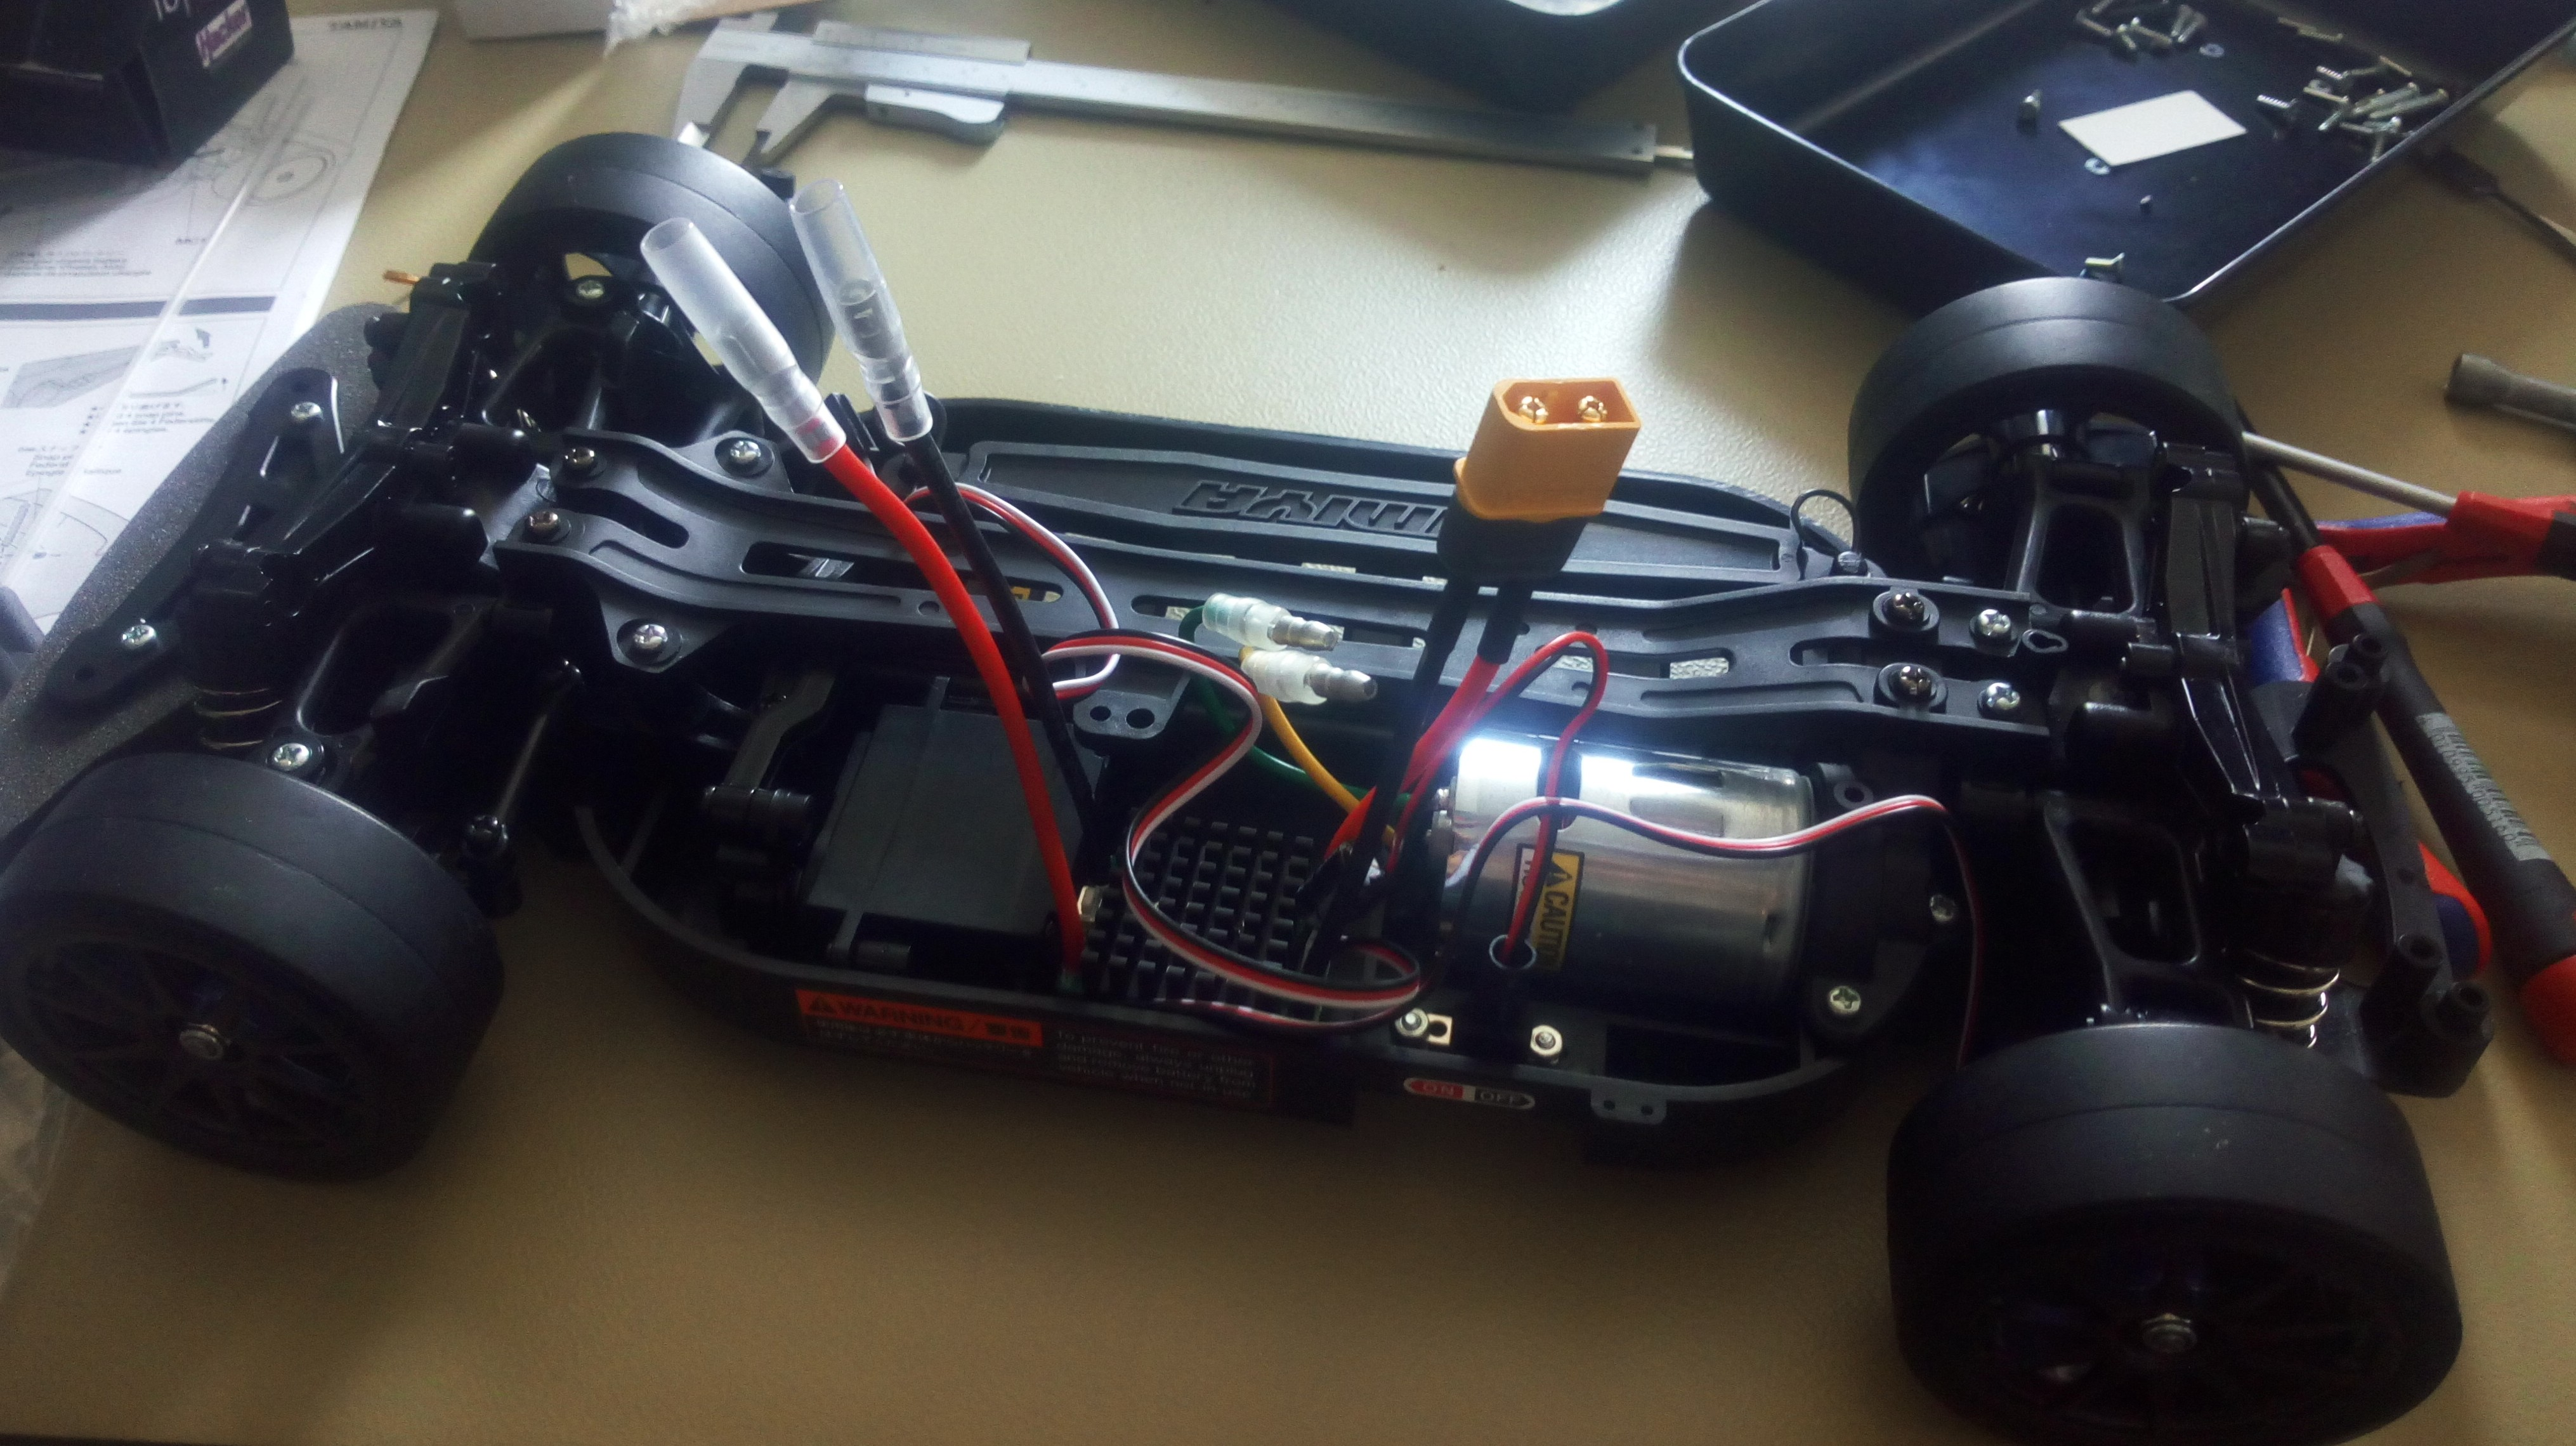
\includegraphics[width=\linewidth]{img/car_body.jpg}
	\caption{Modell Auto und Motoren}
	\label{fig1: Karosserie}
	\end{subfigure}
	\begin{subfigure}[b]{0.4\linewidth}
	\includegraphics[width=\linewidth]{img/Vorne_roboter_vortschritt.jpg}
	\caption{Steuerungselemente}
	\label{fig2: Raspi}
	\end{subfigure}
\end{figure}

Der Roboter wird nach der open source Vorlage von \textit{Donkey Cars} gebaut. (https://docs.donkeycar.com/guide/build\_hardware/ ) Das Donkey Car Projekt benutzt einen Raspberry pi und ein Ferngesteuertes Modellauto um einen Roboter zu bauen. Dazu werden die mechanischen Teile des Autos, ein DC Antriebsmotor, ein Servomotor für die Lenkung und der Akku und Fahrtenregler verwendet. Zusätzlich zum Raspberry Pi wird ein "Motorshield" verwendet. Das ist eine kleine Platine mit einem \textit{PCA9685 16-channel, 12-bit PWM Fm+ I2C-bus LED controller}. Wir steuern Motoren nicht LED Lämpchen. Die Platine sorgt dafür das die die Geschwindigkeit der Motoren gesteuert werden kann und es sorgt dafür das sie  mit der passenden Spannung versorgt werden\\

Zusätzlich wird ein \textit{UBEC} verbaut um den Raspberry Pie sicher mit 5 Volt zu versorgen. Das ist nötig weil der Akku 7 Volt liefert, was den Raspberry Pi beschädigen würde.\\

Eine Raspberry Pi Kamera und ein Ultraschall Sensor sind auch auf dem Roboter verbaut damit der Roboter auf seine Umwelt reagieren kann.

Der Ultraschall Sensor wird mit Hilfe eines Arduinos gesteuert, der per Serieller Schnittstelle mit dem Raspberry Pi Verbunden ist. 

\subsection{Software}

Der source code des Projekts liegt auf \textit{https://github.com/Wifi-cable/Robotic\_AI\_student\_project}. Das Reposatory wurde von  Tiziano Fiorenzani geklont. Die Dokumentation seines Projekts ist auf Youtube. \textit{https://youtu.be/iLiI\_IRedhI} .

\subsubsection{Grobschema}
(Hier fehlt noch ein Bild)
Die Software basiert auf ROS dem Robot Operating system. Sie ist Verteilt, ein Teil wird auf dem Raspberry Pi des Roboters ausgeführt, ein teil auf dem Arduino und ein Teil auf einem Laptop.  Der Raspberry Pi öffnet einen accespoint, mit dem sich ein externer Computer oder Laptop verbindet. Über den computer kann der Roboter Ferngesteuert werden. Der Raspberry Pi wird über die Serielle Schnittstelle vom Arduino mit Sensordaten versorgt. 

\subsubsection{Software architektur}

\begin{figure}[h]
	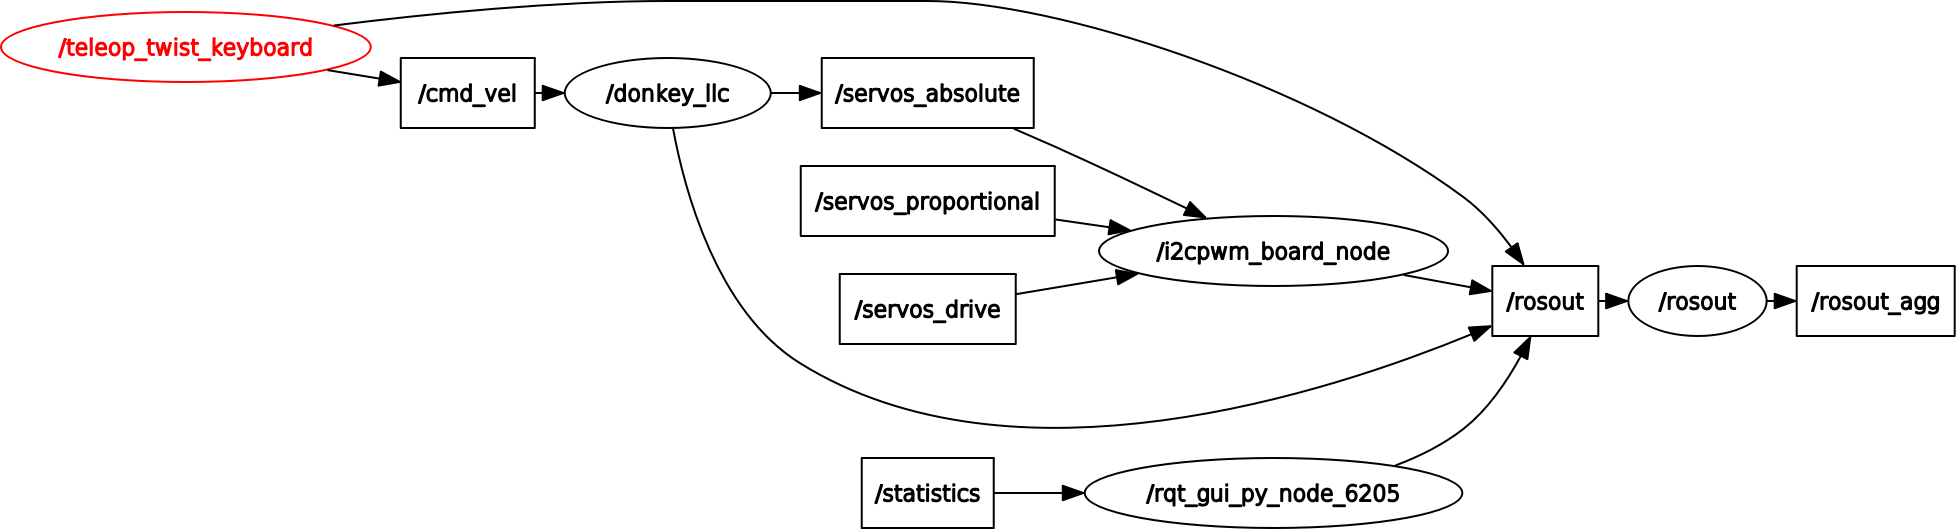
\includegraphics[width=\linewidth]{img/Robot_auto_RQT.png}
	\caption{Grah der ROS Elemente ausgegeben von dem ROS Programm rqt\_graph}
	\label{fig3: RQT}	
\end{figure}

Treu den Prinzipien von ROS besteht die Software aus vielen einzelnen Komponenten genant ROS Nodes. Diese Nodes erledigen immer nur kleine aufgaben. Sie kommunizieren mit Hilfe von ROS Messages(Nachrichten) durch verschiedene ROS Topics (Kanäle für Nachrichten).\\
Die Nodes sind:
\begin{itemize}
	\item roscore (master) 
	\item teleop\_twist\_keyboard (vernsteuerung)
	\item donkey\_llc (Hardware nahe steuerungs Node)
	\item i2cpwm\_board\_node ( Bibliothek und Node um das I2C protokoll zu sprechen und mit ROS zu verbinden)
\end{itemize}
\par
Die Nodes sind durch Topics verbunden durch die sie Nachrichten austauschen. Der genaue Aufbau ist in der abbildung zu sehen des Projects sind: 
\begin{itemize}
	\item cmd\_vel (comand Velocity, die Beschleunigungssteuerung) 
	\item servos\_absolute (Verbindung der Motoren mit den Hardware adressen?)
	\item servos\_proportional (Motorsteuerung für Geschwindigkeit?)
	\item servos\_drive ( Lenken?) 
	\item rosout (Standart ROS output)
\end{itemize}


\subsubsection{Launch Reihenfolge}


\begin{lstlisting}[label={list:first},caption=Sample rosBash code.]
#network ubiquityrobot03B
#connect via SSH
ssh ubuntu@10.42.0.1
#enter password

#on raspi
cd catkin_ws/Robotic_AI_student_project/
source devel/setup.bash
rosrun i2cpwm_board i2cpwm_board 

#second terminal 
#connect via SSH
ssh ubuntu@10.42.0.1
#enter password
cd catkin_ws/Robotic_AI_student_project/
source devel/setup.bash
rosrun donkey_car low_level_control.py

#on laptop
export ROS_MASTER_URI=http://ubiquityrobot.local:11311

roslaunch donkey_car keyboard_demo.launch
\end{lstlisting}



\end{document}